%\part{Aspectos Gerais}

\chapter[Referencial Teórico]{Referencial teórico}
	
	Parte da teoria relacionada à robótica móvel e à robótica educacional será descrita, brevemente, ao longo deste capítulo, visando facilitar o entendimento dos termos utilizados durante a realização desta pesquisa. 

\section{Robótica e a auto-localização}

O nascimento da robótica se deu no contexto industrial, onde a automação de atividades repetitivas garantiu maior eficiência e, consequentemente, maior lucro \cite{roboticaIndustrial}. Porém, com o passar dos anos, a robótica vem se expandindo e fazendo parte da vida cotidiana de muitos \cite{teachingWithRoboticKit}. A robótica é uma importante ferramenta que apóia o trabalho humano em diversos contextos, seja para a limpeza de uma casa \cite{melhoramentoServicoLimpeza} ou até para explorar novos planetas, por exemplo \sloppy \cite{explore_marte}.

No contexto da robótica móvel, existem, por exemplo, os robôs de serviço. Esses robôs vêm sendo largamente evoluídos pela comunidade de robótica \cite{theCleaningProject}. Ainda segundo \cite{theCleaningProject}, estes robôs, geralmente, desempenham ações que contemplam aplicações, como:

\begin{itemize}
	\item Aplicações que envolvam risco de vida significativo para humanos \cite{explore_marte};
	\item Funções economicamente desvantajosas no uso de trabalhadores humanos \cite{roboticaIndustrial};
	\item Uso humanitário (cadeiras de rodas autônomas, por exemplo);
	\item Uso educacional \cite{teachingToolsState-Art}.
\end{itemize} 

Robôs de serviço capazes de se deslocar livremente pelo ambiente, conhecendo-o, poderão realizar suas atividades de forma mais eficiente \cite{theCleaningProject}, o que garante sua autonomia.

Segundo \cite{roboticaIndustrial}, a palavra \textit{automação} traz à mente a noção de que a máquina será capaz de sentir e interagir com o ambiente, conseguindo se localizar e navegar por ele, executando suas atividades. Para que esta navegação seja possível, o robô precisa obter informações sobre o ambiente, as quais são obtidas a partir da utilização de sensores \cite{simpleMobile}. Segundo \cite{agenteExploratorioKalman}, existem inúmeros tipos de sensores, desde sensores de toque até sensores de visão ou de som. Os sensores mais utilizados em robôs móveis, segundo \cite{agenteExploratorioKalman}, são:
\begin{itemize}
	\item \textit{Odômetro}:

		São sensores de implementação simples e de baixo custo. Este tipo de sensor conta a quantidade de rotações de cada roda do robô, o que permite calcular o trajeto percorrido pelo mesmo. Esta técnica é conhecida como \textit{dead-reckoning}, como é apresentado por \cite{integrationVisionSLAMnonlinear}. Segundo \cite{agenteExploratorioKalman}, técnicas como o \textit{dead-reckoning} são bastante suscetíveis a erros, graças ao não alinhamento das rodas, derrapagens das mesmas e até erros no sinal dos sensores.

	\item \textit{Câmera}:

		A utilização de câmeras pode ser bastante útil quando se deseja navegar em um ambiente fechado, construído pelo homem e com características bem definidas, como afirma \cite{agenteExploratorioKalman}. Porém, sua utilização possui uma exigência computacional \cite{localizacaoEMapeamentoPaulo} que muitas vezes pode inviabilizá-la.

	\item \textit{Sonar}:

		É um tipo de sensor de proximidade barato e de fácil utilização e, por esse motivo, é bastante utilizado em robôs móveis para ambientes fechados \cite{agenteExploratorioKalman}. Ainda segundo \cite{agenteExploratorioKalman}, em ambientes abertos, este é um sensor falho, devido ao seu alcance limitado e por não ser direcionado.

	\item \textit{Infravermelho}:

		É um tipo de sensor muito semelhante aos sonares, porém, estes são direcionados, ou seja, são capazes de identificar a direção do objeto \cite{theCleaningProject}.

	\item \textit{Laser}:

		Também é um tipo de sensor semelhante aos sonares e sensores de infravermelho, entretanto, esses, além de serem direcionados, são mais precisos. Tal característica os tornam equipamentos mais caros, como apresenta \cite{agenteExploratorioKalman}.

\end{itemize}

A utilização de cada tipo de sensor se dá de acordo com o contexto em que se deseja navegar, levando em consideração a maneira mais viável de entender o ambiente ao seu redor \cite{agenteExploratorioKalman}. Utilizando os sensores, o robô obterá informações sobre o ambiente, e precisa processá-las para \textit{entender} o mesmo. A maneira de processar (analisar) essas informações também depende do contexto da navegação, como mostra \cite{roboBulldozerIV}.

Para que a navegação ocorra sem colisões em obstáculos, o robô precisa, além de informações sobre o ambiente, informações relacionadas a sua posição em relação a este ambiente \cite{theCleaningProject}. Para solucionar este problema, uma técnica bastante difundida é a utilização de mapas, como mostra \cite{roboBulldozerIV}. Nesta técnica, o robô recebe o mapa do ambiente que se deseja navegar a prióri e, a partir deste mapa, traça sua trajetória sem obstáculos. Utilizando este mapa e informações do ambiente, o robô é capaz de se auto-localizar no ambiente, navegando com maior precisão \cite{roboBulldozerIV}.

Por outro lado, esta técnica possui requisitos que, muitas vezes, são inviáveis, como o conhecimento prévio do mapa do ambiente. Caso o objetivo seja navegar em um ambiente desconhecido, onde não há mapa nem pontos de referência já conhecidos, deve-se buscar formas de se auto-localizar e navegar utilizando apenas as informações obtidas pelos sensores. Para isso, vem sendo discutida na comunidade de pesquisadores em robótica móvel, a resolução do problema de SLAM (Auto-Localização e Mapeamento de Ambientes Simultâneos). Segundo \cite{slamProblem}, SLAM é considerado, pela comunidade, como o \textit{Santo Graal} da robótica móvel.

%----------------------------O PROBLEMA DE SLAM-------------------------------------
\section{O problema de SLAM} % (fold)
\label{sec:section_name}

Auto-localização e Mapeamento de Ambientes Simultâneos (SLAM) é uma técnica bastante utilizada para navegação em diferentes contextos, como na navegação marítima, por exemplo \cite{slamProblem}. Esta técnica garante a possibilidade do robô navegar em um ambiente desconhecido, construindo um mapa do ambiente e, simultaneamente, utilizar este mapa para se auto-localizar em relação ao ambiente \cite{slamProblem}. Ou seja, a técnica de SLAM, utilizando conceitos de inteligência artificial, garante autonomia móvel à maquina.

Segundo \cite{slamProblem}, uma máquina capaz de partir de um ponto de origem desconhecido em um ambiente desconhecido e, utilizando seus sensores, mapear o ambiente, utilizando este mapa, simultaneamente, para se auto-localizar no ambiente faz juz à palavra \textit{robô}. Desse modo, com a vontade de criar verdadeiros \textit{robôs}, pesquisadores em robótica móvel vêm desenvolvendo e evoluindo diversas soluções para o problema de SLAM, nos mais diferentes contextos \cite{integrationVisionSLAMnonlinear}. Esta busca por uma solução elegante ao problema de SLAM possui o intuito de maximizar a efetividade da navegação autônoma \cite{theCleaningProject}. 

A possibilidade de se auto-localizar em um ambiente garante façanhas importantes para a robótica, como a resolução do problema do \textit{sequestro do robô}, por exemplo, como mostra \cite{sequestro}. Este é um problema especial de localização global no campo da robótica móvel, onde o desafio deste problema, segundo \cite{sequestroRobo}, é fazer com que o robô seja capaz de se localizar em um mapa após ser sequestrado.

A ocorrência do \textit{sequestro} se dá quando, o robô, enquanto navega em um ambiente, é retirado do seu local e levado a outro totalmente desconhecido \cite{sequestro}. Em uma situação normal, o robô não seria capaz de entender que não está mais no local onde estava, fazendo com que o mesmo se perdesse. Diversas técnicas para solucionar este problema já foram desenvolvidas, geralmente utilizando como apoio o filtro de partículas, que será apresentado mais à frente \cite{sequestroRobo}. 

De acordo com \cite{circumventingAssociationSLAM}, graças à natureza imperfeita presente nos sensores, à falta de previsibilidade em ambientes reais de atuação e à necessidade de aproximações para viabilizar a análise de decisões computacionais, a robótica é uma ciência dependente de algoritmos probabilísticos. Desse modo, as diversas soluções desenvolvidas, geralmente, diferem umas das outras pela utilização dos algoritmos probabilísticos. Entre os algoritmos mais utilizados, destacam-se o \textit{filtro de kalman} e o \textit{filtro de partículas}, como mostram as seções \ref{sub:kalman} e \ref{sub:filtro_de_partículas}.

\subsection{Filtro de Kalman} % (fold)
\label{sub:kalman}

De acordo com \cite{slamProblem}, a abordagem probabilística mais utilizada para resolução do problema de SLAM é a utilização do filtro de Kalman. \cite{theCleaningProject} descreve o filtro de Kalman como: \textit{"Um algoritmo recursivo de processamento de informações, proporcionando a estimação ótima do estado de um sistema dinâmico com ruído linear"}. Sua utilização está representada de forma clara na Figura \ref{img:kalmanModelagem}.

\begin{figure}[H]
	\centering
	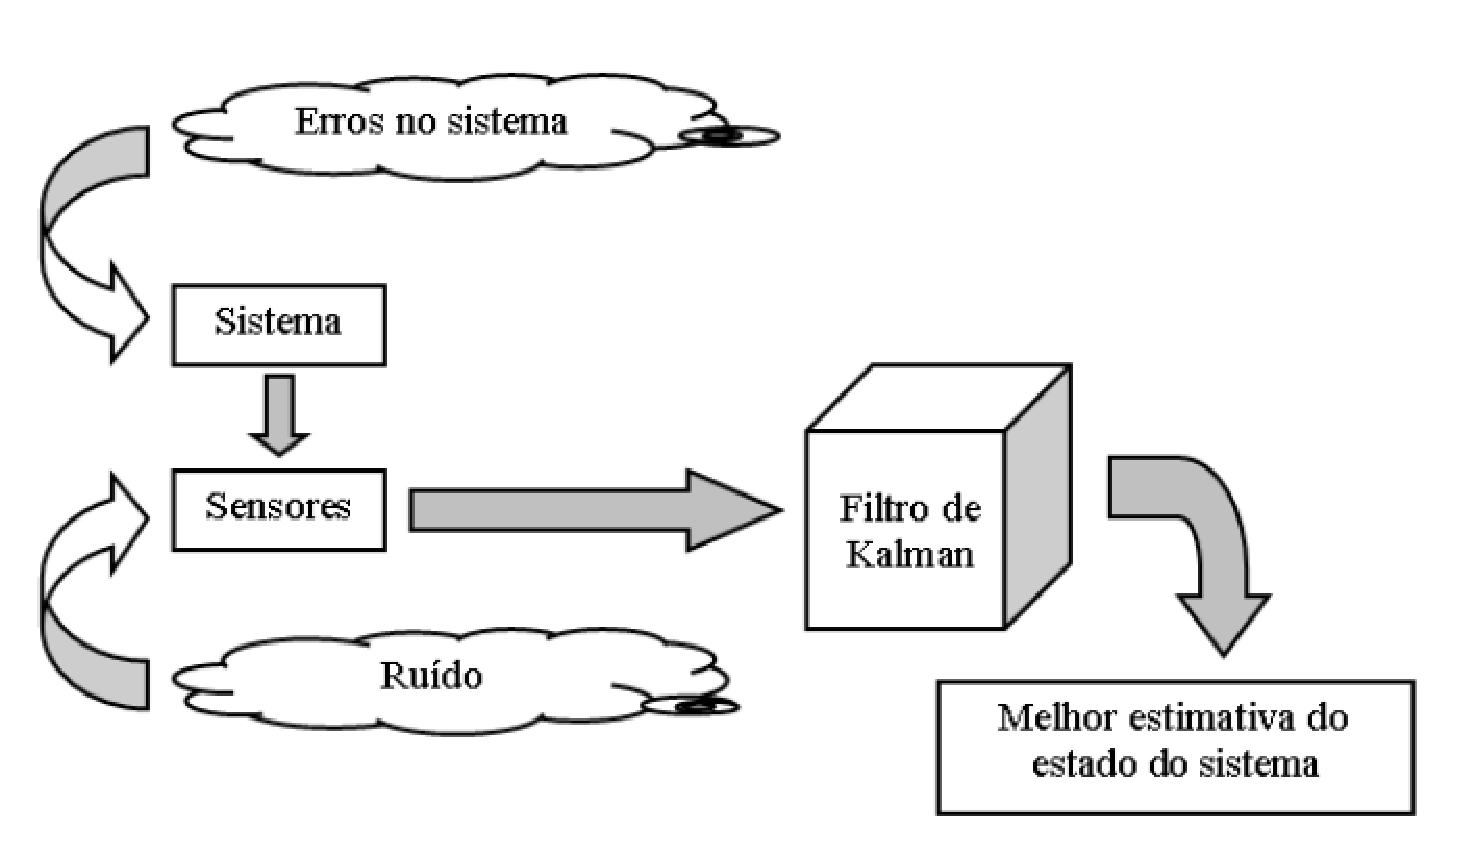
\includegraphics[scale=0.6]{figuras/kalmanModelagem.eps}
	\caption[Utilização do filtro de Kalman]{Utilização do filtro de Kalman. Fonte:\cite{agenteExploratorioKalman}.}
	\label{img:kalmanModelagem}
\end{figure}

Como mostra \cite{theCleaningProject}, entre as disciplinas presentes na utilização deste filtro, encontram-se:
\begin{itemize}
	\item Mínimos quadrados;
	\item Teoria das probabilidades;
	\item Sistemas dinâmicos;
	\item Sistemas estocásticos, e
	\item Álgebra.
\end{itemize}

Apesar das colocações, a utilização da abordagem do filtro de Kalman, geralmente, exige requisitos computacionais de alto custo, dificultando sua utilização em um contexto de robôs simples, onde baixo processamento e pouca memória fazem parte da realidade \cite{agenteExploratorioKalman}.

 Em seu trabalho, \cite{slamProblem} exemplifica este problema, quando quantifica a relação entre o crescimento do requisito computacional necessário para a quantidade de pontos de referência no ambiente, com a utilização do filtro de Kalman. Segundo ele, enquanto a quantidade de pontos de referência aumenta em N, os requisitos computacionais e de armazenamento necessários aumentam em N\textsuperscript{2}. \cite{slamProblem} mostra que este problema pode ser solucionado, em parte, utilizando técnicas de aproximação delimitada, por exemplo. Entretanto, estas técnicas minimizam o problema, mas não o solucionam completamente \cite{slamProblem}.

 % subsection subsection_name (end)

 \subsection{Filtro de partículas} % (fold)
 \label{sub:filtro_de_partículas}

Outra abordagem bastante utilizada para resolução do problema de SLAM envolve a utilização do filtro de Partículas, que é uma técnica para implementação de um \textit{Filtro Bayesiano} de forma recursiva, utilizando o método de \textit{Monte Carlo} \cite{integrationVisionSLAMnonlinear}. O método de Monte Carlo baseia-se em amostragens aleatórias em grande quantidade com o objetivo de estabelecer o valor de uma grandeza que não é disponível através de uma expressão matemática \cite{mooney1997monte} e \cite{comparacaoKalmanParticulas}.

O funcionamento desta abordagem baseia-se em subdividir o ambiente em partículas espalhadas uniformemente, que representam o robô munido de seus sensores \cite{comparacaoKalmanParticulas}. Cada partícula é uma hipótese da posição atual do robô \cite{dp-slam}. O robô e as partículas obtêm informações do ambiente; o robô utilizando seus sensores e as partículas utilizando equações matemáticas para geração destes dados \cite{comparacaoKalmanParticulas}. As informações obtidas pelo robô real são comparadas com as informações de cada partícula, excluindo as partículas que não oferecem informações semelhantes às do robô real \cite{comparacaoKalmanParticulas}. Com o passar dos ciclos, as partículas que ainda continuam no ambiente representam a posição atual do robô \cite{comparacaoKalmanParticulas}.

A partir da comparação entre estas duas abordagens (filtro de Kalman e filtro de Partículas) \cite{comparacaoKalmanParticulas}, observou-se que as duas possuem vantagens e desvantagens. O filtro de Kalman converge mesmo com um estado inicial impreciso, fornecendo informações sobre as incertezas presentes em cada estágio e permitindo, ainda, a incorporação de toda informação disponível (sensores) para minimizar a margem de erro da estimativa \cite{comparacaoKalmanParticulas}. Porém, ele só garante a efetividade da estimativa para sistemas lineares com ruídos gaussianos \cite{comparacaoKalmanParticulas}. O mesmo não resolve o problema do \textit{sequestro do robô}, apresentado anteriormente.

Já o filtro de Partículas, permite sua utilização em sistemas sem ruído gaussiano, e soluciona o problema do sequestro do robô \cite{filtroParticulasComLEGO}. Entre suas desvantagens, encontram-se o custo computacional e a dificuldade da definição da quantidade ideal de partículas a serem utilizadas \cite{comparacaoKalmanParticulas}.

% subsection filtro_de_partículas (end)

As duas abordagens apresentadas anteriormente são amplamente utilizadas em diversos contextos do mundo real, contemplando questões importantes a serem estudadas e refinadas por estudiosos de engenharia de todo o mundo, desde estudantes que buscam ingressar nesta área até profissionais da área \cite{simpleRobotsIntroductionEng}. Desse modo, vê-se a necessidade da adaptação de técnicas de resolução do problema de SLAM, seja a partir de uma abordagem baseada no filtro de Kalman, ou de uma abordagem baseada no filtro de Partículas, para um contexto Educacional. Nesse contexto, sensores, capacidades de processamento e memória são bastante limitados \cite{roboticEducationBasedLego}.
% section section_name (end)

%---------------------------------ROBÓTICA EDUCACIONAL------------------------------------
\section{Robótica educacional} % (fold)
\label{sec:robótica_educacional}

A utilização da robótica como uma ferramenta de apoio ao aprendizado vem sendo ampliada com o passar dos anos \cite{teachingWithRoboticKit}. Principalmente, graças ao reconhecimento, por muitos autores, dos benefícios da utilização destas tecnologias como abordagem de ensino, onde os alunos são inseridos no problema real e instigados a solucioná-lo \cite{teachingWithRoboticKit}, \cite{construcionismoPapert}, \cite{roboticaEducativaEnsinoMedio}.

Entre os benefícios apresentados por \cite{daMaquinaDeEnsinarAMaquinaDeAprender} e \cite{PCsEConstrucionismo}, pode-se destacar, o maior interesse dos alunos sobre o tema, a abordagem facilitadora para o relacionamento entre aluno, professor e conteúdo, a experiência com trabalho em grupo, a multidisciplinariedade e a construção do conhecimento por parte do aluno.

Referente ao aperfeiçoamento do interesse dos alunos sobre o tema, \cite{construcionismoPapert} e \cite{teachingWithRoboticKit} apresentam motivos deste aperfeiçoamento, como:
\begin{itemize}
	\item Curiosidade sobre a tecnologia;

	\item Reconhecimento do problema real como um problema cotidiano do aluno, e

	\item Utilização do princípio \textit{Hands-on} \cite{PCsEConstrucionismo}
\end{itemize}

Sobre o aperfeiçoamento da relação entre alunos, professor e conteúdo, \cite{construcionismoPapert} destaca a reformulação do padrão de ensino e aprendizagem durante a aula. De acordo com \cite{construcionismoPapert}, no contexto do ensino tradicional, o aluno busca \textit{clonar} o conhecimento do professor, decorando informações para, no futuro, utilizá-los no contexto real. \cite{roboticaEducativaEnsinoMedio} acrescenta que, esta abordagem, além de limitar o aprendizado do aluno ao conhecimento do professor, minimiza a capacidade de aprendizado do aluno, já que o conhecimento não é construído, e sim repassado.

Já na abordagem da utilização de tecnologias no contexto educacional, a resolução prática do problema atacado faz com que alunos e professores trabalhem lado-a-lado, muitas vezes realizando troca de papéis aluno/professor, como apresentam \cite{construcionismoPapert} e \cite{daMaquinaDeEnsinarAMaquinaDeAprender}. Desse modo, em muitas ocasiões, os alunos se encontram explicando uma possível solução do problema ao professor, o que acaba com o aprendizado limitado ao conhecimento do professor \cite{PCsEConstrucionismo}. \cite{construcionismoPapert} caracteriza o professor como um fio condutor do conhecimento, e não a fonte do mesmo.

Já, de acordo com a relação da experiência do aluno em trabalhos em grupo, a abordagem \textit{Hands-on} garante que todos os envolvidos na solução devem interagir entre si, trocando conhecimento e ideias \cite{teachingWithRoboticKit}. Qualquer contexto em que se deseja trabalhar, atualmente, envolve inúmeras atividades de trabalho em grupo \cite{teachingWithRoboticKit}. Desse modo, o aperfeiçoamento da capacidade de trabalhar em grupo é uma atividade essencial para o futuro profissional do aluno \cite{PCsEConstrucionismo}.

Outra característica importante da utilização da tecnologia como ferramenta de aprendizado é a multidisciplinariedade \cite{analiseFerramentaEnsinoComputacao}, já que conteúdos referentes a diversas disciplinas são trabalhados e adaptados para buscar a solução do problema em investigação. \cite{teachingWithRoboticKit} sugere a utilização de atividades multidisciplinares para aprendizado de conteúdos base, como matemática e física, minimizando o problema do conhecimento parcial de certos conteúdos.

Além de todos os benefícios apresentados acima, uma forte qualidade da abordagem \textit{Hands-on} é referente à construção do conhecimento por parte do aluno \cite{PCsEConstrucionismo}. Esta construção é gerada utilizando conhecimentos básicos de diferentes disciplinas para solucionar um problema que exige a integração de diversos conteúdos, seguindo uma filosofia construcionista, como é apresentado por \cite{construcionismoPapert}.
 
%\subsection{Construcionismo} % (fold)
%\label{sub:construcionismo}

	De acordo com \cite{construcionismoPapert}, quando o aluno se sente imerso no problema trabalhado, a maneira com que o mesmo aprende é aperfeiçoada, maximizando as relações entre aluno, professor e conteúdo. Este pensamento segue uma filosofia construcionista, a qual, de acordo com \cite{construcionismoPapert}, implica no objetivo de ensinar, de forma a produzir o máximo de aprendizagem a partir do mínimo de ensino.

	A utilização de aplicações rotineiras do mundo real é uma forma bastante eficaz de obter máximo interesse dos alunos nos conteúdos apresentados \cite{construcionismoPapert}. Desse modo, inserir alunos na resolução de problemas presentes no contexto da robótica móvel, por exemplo, fará com que os mesmos aprendam, com eficiência, diversos temas recorrentes no contexto mundial da robótica móvel \cite{simpleRobotsIntroductionEng}, além de conteúdos presentes em diversas disciplinas, como matemática e física \cite{roboticaEducacionalAulasMatematica}.

	O construcionismo é baseado em uma filosofia construtivista \cite{construcionismoPapert}, que afirma que o conhecimento não deve ser uma cópia da realidade, e sim uma construção, realizada pelo aluno a partir da sua interação com o contexto do problema \cite{oQueEConstrutivismo}.

% subsection construcionismo (end)

Segundo \cite{simpleRobotsIntroductionEng}, a utilização da robótica no meio da educação traz inúmeros benefícios que vão além dos objetivos diretos da melhoria da aprendizagem. De acordo com ele, sua utilização garante a introdução dos estudantes nos problemas recorrentes do contexto de Engenharia mundial. Esta introdução possui grande importância para a evolução do país, já que a demanda por profissionais qualificados na área de Engenharia, no mundo atual, é ampla \cite{simpleRobotsIntroductionEng}. De acordo com \cite{analiseFerramentaEnsinoComputacao}, em 2014 no Brasil, haviam cerca de 78 mil vagas relacionadas à área de Tecnologia da Informação e apenas 33 mil foram preenchidas, o que comprova a falta de profissionais na área.  \cite{analiseFerramentaEnsinoComputacao} afirma, ainda, que o motivo para esta falta de profissionais é resultado advindo do baixo interesse por parte dos estudantes brasileiros por ciências exatas.

Grande parte deste baixo interesse, segundo \cite{oQueEConstrutivismo}, é devido à metodologia tradicional de ensino, onde os alunos buscam copiar o conhecimento do professor, sem atividades com abordagem construcionista de aprendizado, por exemplo. Uma forma de aumentar o interesse dos alunos, segundo \cite{roboticaEducacionalAulasMatematica}, é a utilização da robótica como uma ferramenta de apoio ao aprendizado, seguindo uma abordagem construcionista.

Atualmente, de acordo com \cite{analiseFerramentaEnsinoComputacao}, no Brasil, o ensino de computação e robótica se restringe aos níveis superiores e técnicos, exceto alguns projetos realizados por universidades em escolas de nível fundamental e médio, como \cite{projetoRoboticaMauricio}. Esta introdução tem como objetivo introduzir noções lógicas e computacionais na Educação Básica, despertando o interesse dos alunos nas ciências exatas e estimulando-os a ingressar na carreira de Engenharia \cite{analiseFerramentaEnsinoComputacao}.

Diversas ferramentas já foram desenvolvidas com o objetivo de apoiar a inserção de alunos da Educação Básica no contexto da computação e robótica. Na seção \ref{sec:robótica_educacional_suporte}, são apresentadas algumas utilizadas por \cite{analiseFerramentaEnsinoComputacao}, \cite{projetoRoboticaMauricio}, \cite{simpleRobotsIntroductionEng}. Ferramentas como essas, são utilizadas em diversos contextos, desde a utilização como apoio ao aprendizado, como mostra \cite{teachingWithRoboticKit}, até a utilização em campeonatos e jogos, como mostra \cite{ciber-rato}. 

De acordo com \cite{analiseFerramentaEnsinoComputacao}, algumas abordagens utilizam ferramentas virtuais para facilitar o aprendizado. Por outro lado, segundo \cite{simpleMobile}, a utilização de ferramentas reais, equipadas com sensores e atuadores, garante maior interesse e introdução do aluno no contexto da engenharia do mundo real. Desse modo, a ferramenta utilizada neste trabalho será o kit de robótica educacional Mindstorm, da Lego, que tem suas características especificadas na seção \ref{sub:kit_mindstorm}.

\subsection{Lego Mindstorms NXT} % (fold)
\label{sub:kit_mindstorm}

Com o passar dos anos, os componentes de \textit{hardware} vêm sendo evoluídos continuamente \cite{teachingWithRoboticKit}. Esta evolução faz com que o preço de componentes simples tenda a diminuir, como é o caso de pequenos processadores poderosos e praticamente descartáveis \cite{teachingWithRoboticKit}. Desse modo, esta evolução dos componentes de \textit{hardware} vem permitindo a utilização dos mesmos em diversos contextos, como educação e entretenimento. 

Com o crescimento de demandas relacionadas a estes componentes, nascem os kits de robótica que integram componentes simples, porém, poderosos para utilização no contexto educacional e de entretenimento \cite{teachingWithRoboticKit}. Entre os kits existentes atualmente no mercado, destaca-se o kit de robótica Mindstorm, da Lego, o qual foi desenvolvido na década de 80 por pesquisadores do MIT. O kit utiliza peças de montagem no padrão Lego para construir a estrutura do robô, diversos tipos de sensores e alguns atuadores, para garantir a mobilidade e interação com o ambiente \cite{teachingWithRoboticKit}.

Desde o lançamento do kit, na década de 80, o mesmo é utilizado por instituições de ensino como ferramenta de apoio ao aprendizado. O sucesso do kit o garantiu premiações devivo a sua reusabilidade, modularidade e simplicidade, associado ao seu baixo custo \cite{teachingWithRoboticKit}.

O cérebro do kit pode ser observado na Figura \ref{img:cerebro}, onde se encontra um microprocessador disposto de diversos acessos para sensores e atuadores. Em alguns modelos do kit, o cérebro possui uma tela LCD e alguns botões para interação do usuário. Além do cérebro, o kit possui alguns sensores, como o apresentado na Figura \ref{img:sensorLego}, e atuadores, como na Figura \ref{img:atuadorLego}

\begin{figure}[H]
	\centering
	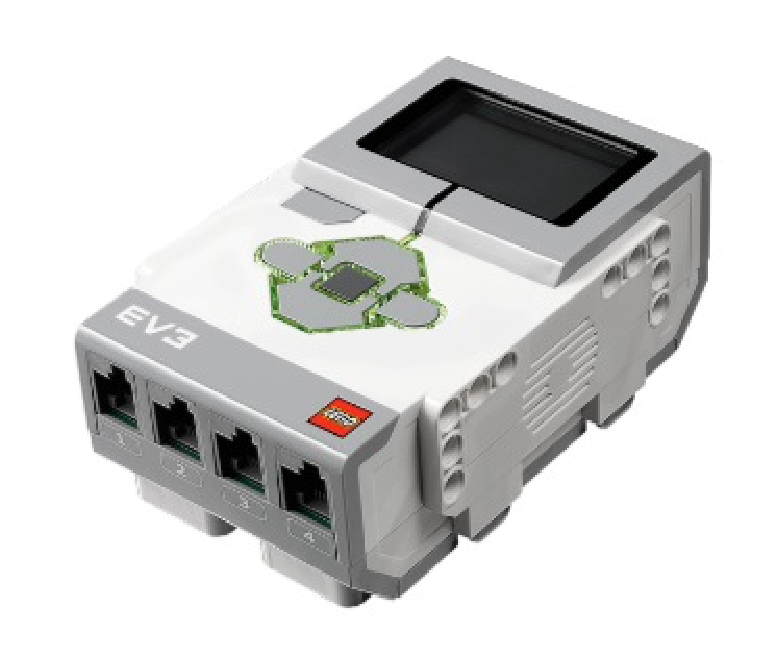
\includegraphics[scale=0.6]{figuras/cerebro.eps}
	\label{img:cerebro}
	\caption[Microprocessador central]{Microprocessador central}
\end{figure}	

\begin{figure}[H]
	\centering
	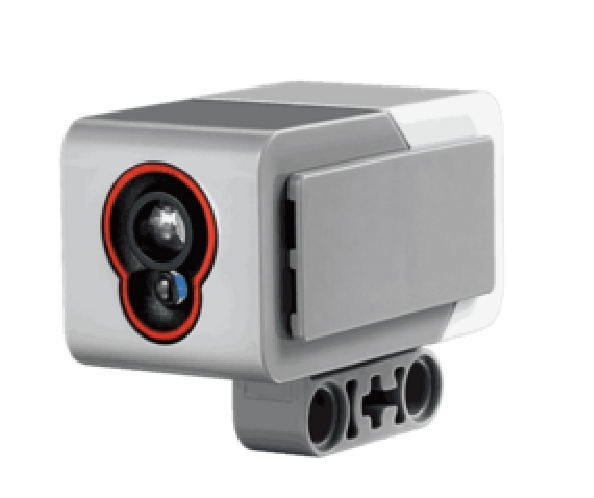
\includegraphics[scale=0.5]{figuras/sensorLego.eps}
	\caption[Sensor RGB - Lego]{Sensor RGB - Lego}
	\label{img:sensorLego}
\end{figure}	

\begin{figure}[H]
	\centering
	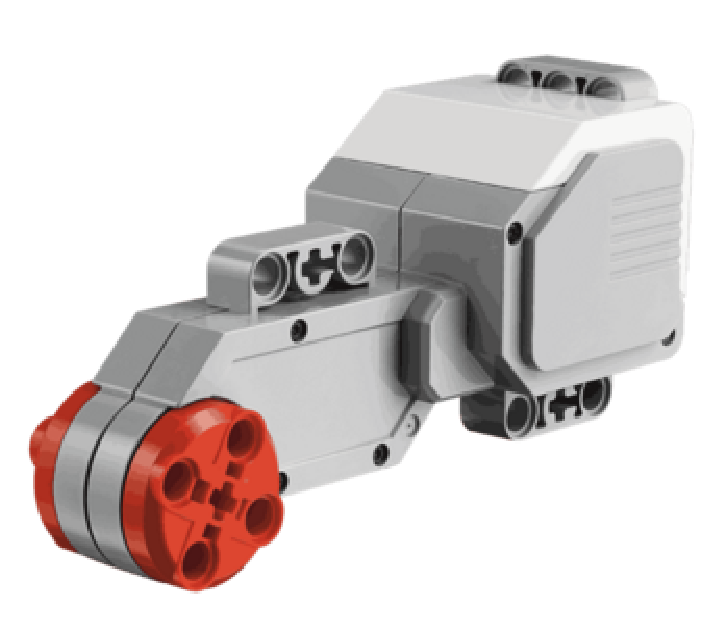
\includegraphics[scale=0.5]{figuras/atuadorLego.eps}
	\caption[Atuador - Lego]{Atuador - Lego}
	\label{img:atuadorLego}
\end{figure}

Além da obtenção do kit completo, como mostra na Figura \ref{img:kit}, é possível adquirir componentes separados, como sensores e atuadores específicos, o que garante a possibilidade de adquirir apenas os componentes necessários para o contexto de aplicação, minimizando os custos da sua utilização.

\begin{figure}[H]
	\centering
	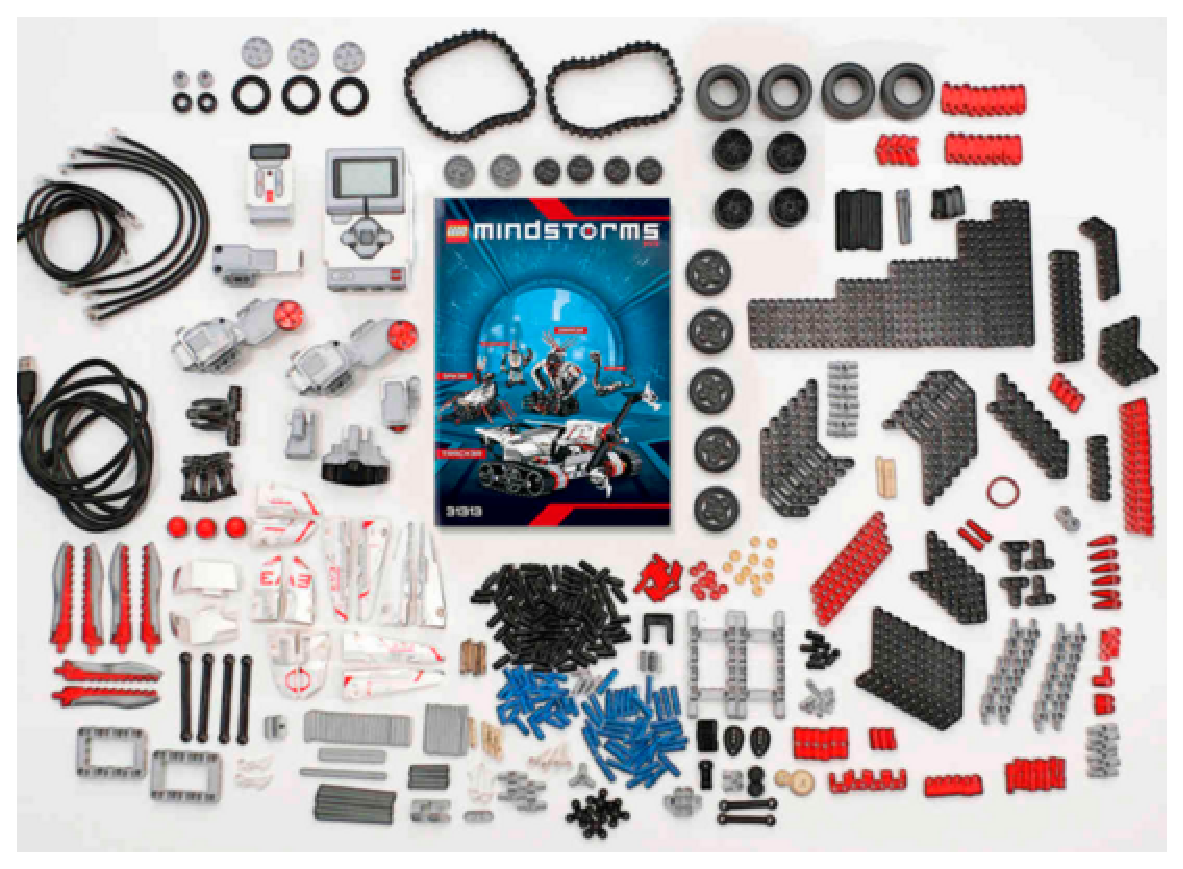
\includegraphics[scale=0.7]{figuras/kitLego.eps}
	\caption[Kit Mindsotm completo - Lego]{Kit Mindsotm completo - Lego}
	\label{img:kit}
\end{figure}


\section{Considerações parciais} % (fold)
\label{sec:considerações_parciais}

	A utilização da tecnologia como ferramenta de apoio ao aprendizado, como foi apresentado durante o capítulo, garante diversos benefícios ao aluno e até ao professor. Principalmente, quando o contexto trabalhado envolve problemas reais da comunidade de robótica, como o problema de SLAM. A partir desta linha de pensamento, este capítulo buscou apresentar informações importantes para viabilizar a compreensão da pesquisa realizada, como a apresentação do problema de SLAM, os filtros probabilísticos mais utilizados e a abordagem educacional da Robótica.

	A partir do conteúdo apresentado durante este capítulo, este trabalho irá buscar aplicar técnicas de auto-localização no contexto limitado da robótica educacional, aproximando os estudos em sala de aula dos contextos da robótica mundial.

% section considerações_parciais (end)
%Mindstorms NXT é uma linha de robótica da Lego, composta de um microcontrolador ARM7 com entrada para até quatro sensores e três atuadores. Possuindo uma tela LCD e botões, a interação com o usuário é de fácil entendimento.
% subsection kit_mindstorm (end)
% section robótica_educacional (end)
